\subsection{Join network \rom{1}}

\begin{figure}[htb!]
  \centering
    \subfloat[]{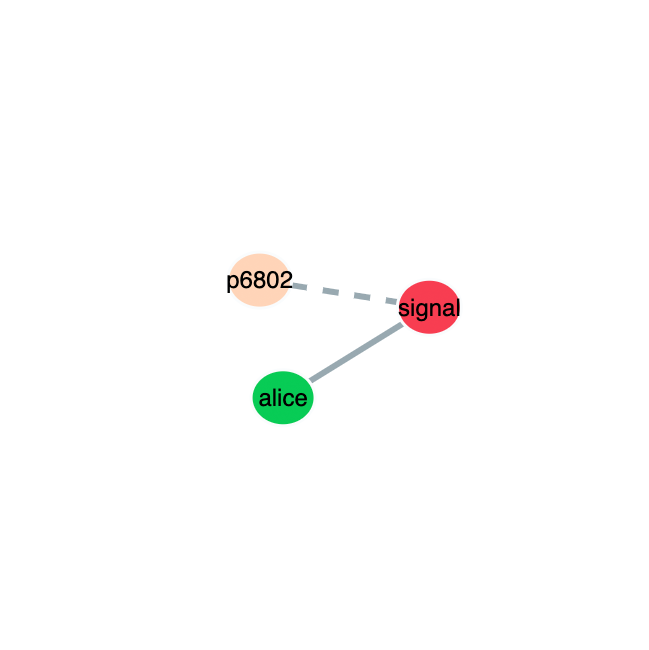
\includegraphics[width=0.25\textwidth]{graphics/analysis/mini-scenarios/join-network/1.png} \label{fig:filmstrips-join-a}}
    \subfloat[]{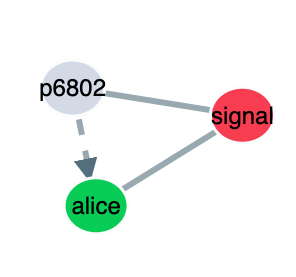
\includegraphics[width=0.25\textwidth]{graphics/analysis/mini-scenarios/join-network/2.png} \label{fig:filmstrips-join-b}}
	\subfloat[]{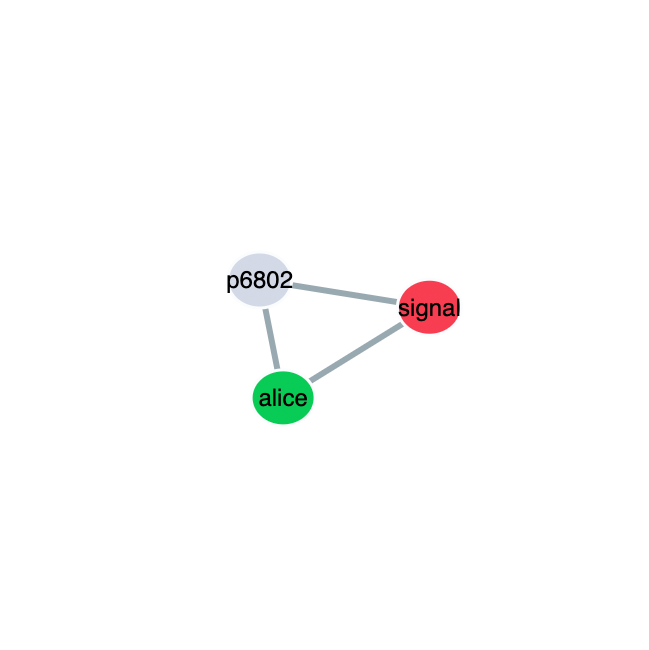
\includegraphics[width=0.25\textwidth]{graphics/analysis/mini-scenarios/join-network/3.png} \label{fig:filmstrips-join-c}}
	\subfloat[]{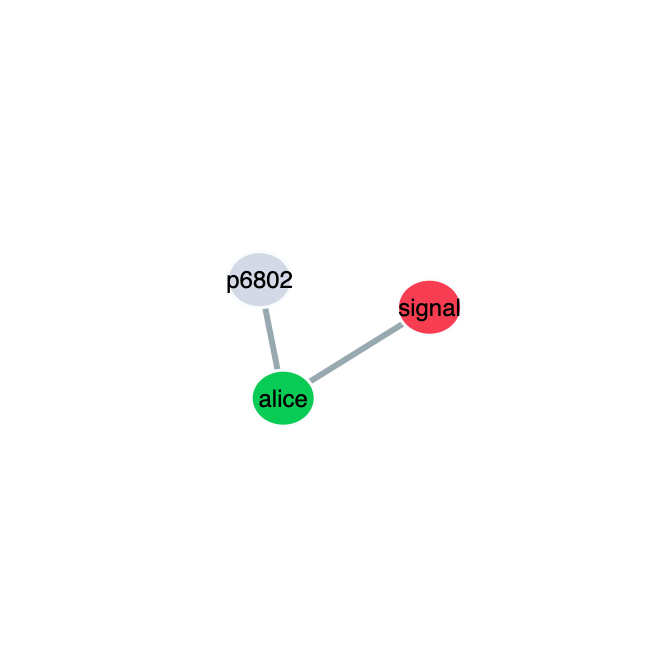
\includegraphics[width=0.25\textwidth]{graphics/analysis/mini-scenarios/join-network/4.png} \label{fig:filmstrips-join-d}}
	\caption{Join network as second peer}
\label{fig:filmstrips-join}
\end{figure}

In this scenario a second peer is joining the network. As described in the in the \textit{Genesis} scenario it opens a connection to the \signal peer (\vref{fig:filmstrips-join-a}). This time the \signal peer already knows a \router peer—\alice. Therefore, it only upgrades the \newbie peer to the role \peer. Also it sends a \peerUpdate to the new peer in order to let it update its peer table. 

A peer with the role \peer has always the desire to satisfy its connection goal.
Thus, its next intention is to open connections to as many peers as it knows, until its connection goal is satisfied. As it only knows the reported peer \alice it is trying to connect to her by sending a connection offer via the \signal peer (\vref{fig:filmstrips-join-b}).

\alice has connections available, hence she is accepting the connection offer with an answer, that is again delivered via the \signal. As soon as the new peer receives the answer, it establishes the connection to \alice (\vref{fig:filmstrips-join-c}).

In the last step it closes the connection to the \signal peer because it knows a peer with the role \router (\vref{fig:filmstrips-join-d}).

